\section{Introdução}

\subsection{Contextualização temática}

No campo da inteligência artificial generativa, grandes modelos de linguagem (\textit{large language models} -- LLMs) são modelos capazes de produzir texto em linguagem natural a partir de padrões aprendidos em grandes volumes de dados textuais \parencite{brownEtAl2020fewShotLearners,zhaoEtAl2023llmSurvey,minaee2024llmSurvey}. Apesar dessa capacidade, LLMs não garantem, por si só, confiabilidade factual, atualização ou verificabilidade documental, pois, quando utilizados de forma isolada, podem produzir respostas plausíveis sem correspondência documental verificável, refletir limitações de atualização decorrentes de bases usadas no treinamento e deixar de indicar as evidências que sustentam cada afirmação \parencite{jiEtAl2023hallucinationSurvey,anhHoang2025hallucinations,dahlEtAl2024largeLegalFictions}.

Para mitigar limitações e riscos associados ao uso isolado de LLMs, foi proposta a abordagem \textit{retrieval-augmented generation} (RAG), que combina modelos generativos com mecanismos de recuperação da informação \parencite{lewisEtAl2020rag}. Nessa abordagem, em vez de depender apenas do conhecimento paramétrico incorporado ao modelo, a geração da resposta passa a ser condicionada por documentos recuperados de uma base documental externa \parencite{lewisEtAl2020rag,gao2023ragSurvey}.

Entretanto, o uso de RAG não elimina o desafio relacionado à qualidade e à verificabilidade das respostas; esse desafio passa a depender da arquitetura do sistema, especialmente do \textit{pipeline}, que é formado por diversos componentes, tais como: preparação dos dados, segmentação textual ou \textit{chunking}, qualidade dos metadados, modelo de \textit{embedding}, estratégia de recuperação, seleção, filtragem ou reranqueamento de contexto, desenho do \textit{prompt}, modelo gerador e critérios de pós-processamento \parencite{gao2023ragSurvey,gupta2024comprehensiveRag,gao2024modularRag}. A Figura~\ref{fig:rag-pipeline} apresenta os componentes da arquitetura RAG, cujas configurações podem influenciar, isoladamente ou em conjunto, a qualidade das respostas e das evidências recuperadas.

\begin{figure}[H]
\centering
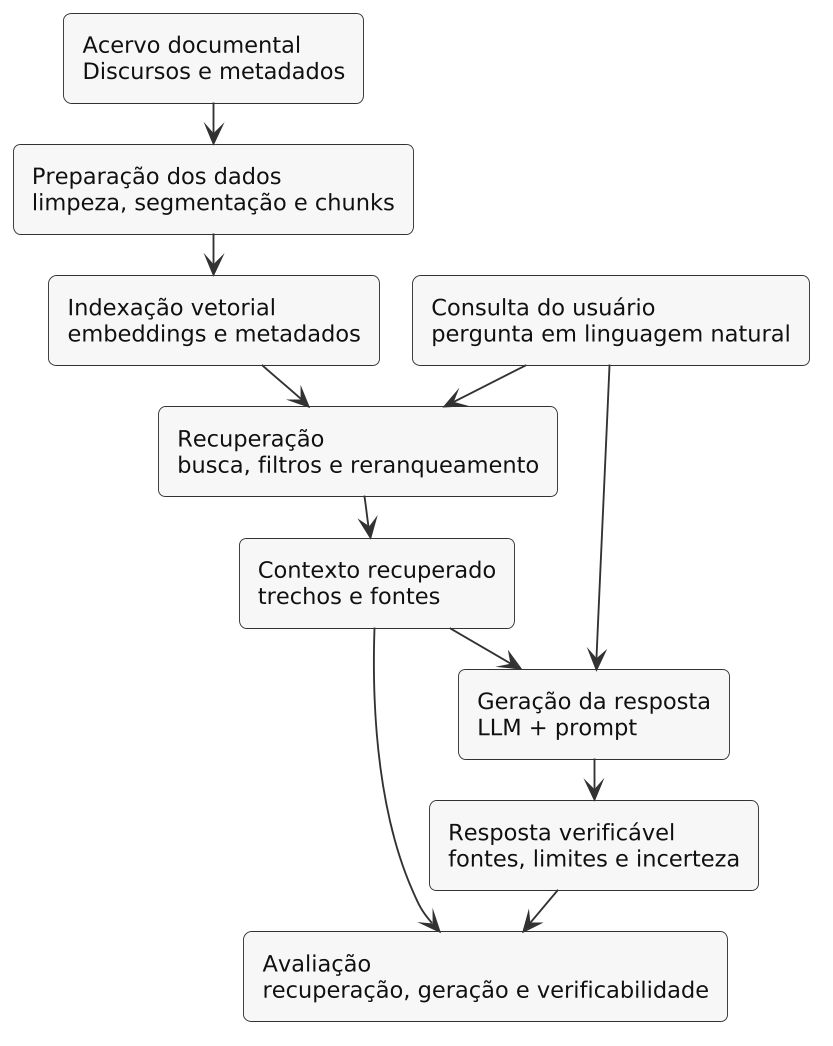
\includegraphics[width=0.88\textwidth]{figures/rag-pipeline.png}
\caption{Componentes de um \textit{pipeline} RAG relevantes para a avaliação de recuperação, geração e verificabilidade}
\label{fig:rag-pipeline}
\par\smallskip
{\small Fonte: elaborado pelo autor.}
\end{figure}

A introdução da arquitetura RAG faz com que a avaliação desses sistemas seja um problema multidimensional, uma vez que não basta examinar a fluência da resposta final; é necessário considerar também como diferentes configurações influenciam a qualidade das respostas e das evidências recuperadas \parencite{liangEtAl2023helm,saadFalconEtAl2024ares,esEtAl2023ragas,pipitoneAlami2024legalbenchRag}. Isso porque uma resposta fluente pode estar apoiada em evidências frágeis; uma recuperação pertinente pode ser mal aproveitada pela geração; e uma avaliação automatizada pode superestimar respostas formalmente plausíveis, mas insuficientemente fundamentadas \parencite{liuEtAl2023geval,liuEtAl2025judgeRag}.

Para enfrentar essa multidimensionalidade, a literatura sobre avaliação de RAG, exemplificada por propostas como RAGAS, ARES e LegalBench-RAG, apresenta técnicas de avaliação complementares \parencite{esEtAl2023ragas,saadFalconEtAl2024ares,pipitoneAlami2024legalbenchRag}. Essas técnicas incluem: métricas de recuperação (como \textit{recall}, \textit{precision}, MRR e nDCG), que medem a pertinência dos documentos recuperados \parencite{manningEtAl2008informationRetrieval,thakurEtAl2021beir}; rubricas de avaliação de geração, que examinam corretude factual, aderência ao contexto e verificabilidade; avaliação humana de respostas, que captura dimensões qualitativas e contextualmente relevantes; avaliação automatizada baseada no paradigma \textit{LLM-as-a-judge}, que permite ampliar a escala de julgamentos, embora exija controle de consistência e critérios explícitos; e análise qualitativa de erros, que revela padrões e casos críticos \parencite{liuEtAl2023geval,liuEtAl2025judgeRag}.

Esse problema avaliativo é especialmente relevante para organizações da administração pública que operam acervos digitais extensos. Nesses ambientes, respostas produzidas por sistemas generativos não podem ser examinadas apenas por fluência ou utilidade aparente. Elas precisam ser verificáveis, rastreáveis, aderentes às evidências recuperadas e compatíveis com requisitos de transparência, responsabilização e supervisão humana \parencite{deAlmeidaSantos2025aiGovernance,wfd2023guidelinesAiParliaments,ipu2024aiParliaments}.

No Poder Legislativo, essas exigências assumem contornos próprios. Discursos parlamentares, debates, proposições, pareceres e demais documentos públicos registram posições políticas, justificativas, argumentos técnicos e trajetórias institucionais que interessam a parlamentares, equipes técnicas, pesquisadores, jornalistas, organizações da sociedade civil e cidadãos \parencite{geunis2023parliamentaryMonitoring,skubicFiser2024discourseReview}. Embora a publicidade desses documentos seja condição necessária para a transparência, ela não garante, por si só, acesso substantivo à informação \parencite{bandeiraBernardes2016information}. Grandes acervos legislativos combinam volume elevado, diversidade temática, dispersão temporal, variação terminológica, autoria múltipla e dependência de metadados, características que desafiam métodos tradicionais de recuperação da informação e também tensionam sistemas RAG \parencite{manningEtAl2008informationRetrieval,skubicFiser2024discourseReview,martelloteViola2025organizacaoConhecimento}.

No Senado Federal brasileiro, os pronunciamentos em plenário constituem um corpus especialmente pertinente para investigar esse problema. Estudos do Núcleo de Estudos e Pesquisas da Consultoria Legislativa indicam que esses registros combinam grande volume documental, variação de extensão, diversidade temática, interatividade e complexidade textual, além de refletirem diferentes usos políticos e institucionais do discurso parlamentar \parencite{blanco2025plenarioPalanqueEstudio,blanco2026letrasGraudas}. Essas características tornam o corpus adequado para uma investigação aplicada sobre avaliação de RAG, pois exigem recuperar evidências em acervo heterogêneo, preservar autoria e contexto, lidar com perguntas de complexidade variável e reconhecer situações em que a informação disponível não sustenta resposta conclusiva.

O tema desta pesquisa, portanto, é o estudo e a aplicação de técnicas de avaliação de sistemas RAG em um sistema voltado à consulta de discursos da 56\textordfeminine{} Legislatura do Senado Federal, recorte escolhido por oferecer delimitação temporal controlada, volume documental expressivo --- aproximadamente 15 mil discursos --- e viabilidade de tratamento empírico do corpus. Esse recorte permite examinar, em condições observáveis, como diferentes técnicas de avaliação podem capturar dimensões complementares da qualidade das respostas e das evidências recuperadas, tais como pertinência das evidências, fidelidade ao contexto recuperado, precisão de autoria, utilidade da resposta, tratamento da insuficiência documental \parencite{esEtAl2023ragas,saadFalconEtAl2024ares,pipitoneAlami2024legalbenchRag}.

\subsection{Apresentação da problemática e da pergunta de pesquisa}

O problema de pesquisa decorre da lacuna quanto a um protocolo articulado para organizar e aplicar técnicas de avaliação de sistemas RAG em domínios institucionais específicos. Essa lacuna será examinada empiricamente a partir de um sistema RAG voltado à consulta de discursos da 56\textordfeminine{} Legislatura do Senado Federal, utilizado como caso empírico para analisar recuperação documental, geração de respostas e verificabilidade das fontes.

Órgãos públicos acumulam acervos de alto valor institucional, mas a adoção de sistemas generativos para explorá-los exige critérios capazes de indicar quando uma resposta é útil, verificável e suficientemente ancorada nas fontes. A literatura sobre RAG já propõe métricas, benchmarks, rubricas, avaliações humanas e estratégias baseadas no paradigma \textit{LLM-as-a-judge}, mas ainda há desafios para organizar essas técnicas em um protocolo aplicável a contextos institucionais específicos, nos quais recuperação, geração e verificabilidade das fontes precisam ser analisadas em conjunto \parencite{gao2023ragSurvey,esEtAl2023ragas,saadFalconEtAl2024ares,liuEtAl2025judgeRag}.

Em contextos jurídico-legislativos, estudos já exploram RAG, LLMs e recuperação semântica em legislação, parlamentos e política, incluindo \textit{fact-checking} político e redação legislativa \parencite{khaliq2024ragar,chouhanGertz2024lexdrafter}, consulta a legislação extensa e interfaces conversacionais \parencite{garrisonEtAl2024talkNdaa,rogiersEtAl2024kamerraad,matoshiEtAl2025parliamentRag}, além de sistemas híbridos com grafos de conhecimento \parencite{colomboEtAl2025legisSearch,mosbachEtAl2025worldAvatarParliament}. No contexto brasileiro, há estudos sobre discursos parlamentares e organização do conhecimento legislativo \parencite{blanco2025plenarioPalanqueEstudio,blanco2026letrasGraudas,martelloteViola2025organizacaoConhecimento}. Ainda assim, permanece lacuna quanto à organização de técnicas de avaliação de RAG, de forma articulada, para analisar recuperação documental, geração de respostas e verificabilidade das fontes em acervos legislativos brasileiros.

Diante disso, formula-se a seguinte pergunta de pesquisa: \textbf{como técnicas de avaliação de sistemas RAG podem ser organizadas e aplicadas à análise da recuperação documental, da geração de respostas e da verificabilidade das fontes em um sistema voltado à consulta de discursos da 56\textordfeminine{} Legislatura do Senado Federal?}

A justificativa prática da pesquisa está na necessidade de avaliar, com critérios explícitos, sistemas generativos aplicados a acervos documentais de interesse público \parencite{wfd2023guidelinesAiParliaments,ipu2024aiParliaments,deAlmeidaSantos2025aiGovernance}. Sistemas RAG podem ampliar a mediação entre usuários e documentos legislativos, mas seu uso institucional exige critérios capazes de indicar quando a resposta está adequadamente ancorada em fontes, quando extrapola o contexto recuperado e quando deve explicitar incerteza ou insuficiência documental. Assim, a contribuição esperada não está em defender a adoção automática de sistemas generativos, mas em oferecer uma forma mais criteriosa de avaliá-los antes de qualquer uso ampliado.

No plano científico, a pesquisa se justifica porque a avaliação de RAG ainda é um campo em consolidação, especialmente quando transposta de \textit{benchmarks} genéricos para domínios públicos específicos. Métricas de recuperação, rubricas de geração, avaliação humana e avaliações baseadas no paradigma \textit{LLM-as-a-judge} medem dimensões complementares, mas nenhuma delas, isoladamente, resolve o problema de verificar qualidade, rastreabilidade e verificabilidade das fontes. Ao tratar o protocolo avaliativo como artefato metodológico aplicado a um sistema RAG em contexto institucional, a dissertação pretende organizar essas técnicas e aplicá-las a um corpus legislativo brasileiro \parencite{hevnerEtAl2004designScience,peffersEtAl2007dsrm}, distinguindo dimensões que, na prática, tendem a aparecer sobrepostas: recuperação documental, geração de respostas, julgamento automatizado, validação humana e verificabilidade das fontes \parencite{esEtAl2023ragas,saadFalconEtAl2024ares,pipitoneAlami2024legalbenchRag}.

\subsection{Enunciação dos objetivos}

\subsubsection{Geral}

Organizar técnicas de avaliação de sistemas RAG em um protocolo articulado e aplicá-lo a um caso empírico de consulta a discursos da 56\textordfeminine{} Legislatura do Senado Federal, com foco na recuperação documental, na geração de respostas e na verificabilidade das fontes.

\subsubsection{Específicos}

\begin{enumerate}
  \item sistematizar a literatura sobre técnicas de avaliação de RAG, incluindo métricas de recuperação, avaliação de geração, benchmarks, rubricas, avaliação humana e avaliações baseadas no paradigma \textit{LLM-as-a-judge};
  \item selecionar, a partir da sistematização da literatura, técnicas de avaliação de RAG a serem aplicadas ao caso empírico, contemplando recuperação documental, geração de respostas e verificabilidade das fontes;
  \item caracterizar o acervo de discursos parlamentares da 56\textordfeminine{} Legislatura do Senado Federal como caso empírico da pesquisa;
  \item construir uma bateria de perguntas de teste, com categorias, respostas esperadas e evidências documentais de referência;
  \item aplicar ao caso empírico o protocolo de avaliação organizado a partir das técnicas selecionadas;
  \item analisar a complementaridade e os limites das técnicas avaliativas quando aplicadas a um acervo legislativo real, com foco na recuperação documental, na geração de respostas e na verificabilidade das fontes.
\end{enumerate}

Em conjunto, esses objetivos conectam três níveis do estudo: a sistematização conceitual das técnicas de avaliação, a organização dessas técnicas em protocolo empírico e a análise dos resultados no contexto do corpus legislativo. Essa sequência busca garantir que a pergunta de pesquisa seja respondida por evidências observáveis, e não apenas por revisão bibliográfica ou demonstração técnica isolada.
